
\subsection{Recipes for engineering templates}
\label{ssec:recipes_technical}

% HB 20230726: We decided that the recipes listed here should be included.
%\TBD It is not clear (2020-11-19) whether data from maintenance
%templates need to be reduced by the pipeline. This section and the
%recipes described therein serves as a placeholder and may be removed
%later.

The CLC coronagraph was removed from the baseline coronagraphic modes before FDR however the coronagraph would be technically available during engineering. At this stage the DRL will not have the corresponding recipes to use the CLC. However, if the need arises during commissioning or after to make the CLC mode available, its DRL recipe can be adapted from the baseline RAVC/CVC coronagraph recipes as it is related in design and usage.

%------------------------------------------------------------------------------------------------------------------
\subsubsection{\REC*{metis_pupil_imaging}: Pupil imaging}\label{rec:metis_pupil_imaging}
\label{sssec:pupil_imaging}

This recipe refers to pupil imaging using the science detectors.
Pupil imaging is needed to verify the alignment and illumination of the pupil masks (part of the HCI coronagraphs) with the telescope beam.
It is not foreseen to be used by scientists in regular operation.

% From OC:
%Presumably it only contains the most basic reduction  steps.
%There may have to be separate recipes for the various
%subsystems.

% From GO:
%Also it can be used to record the pupil transmission which can improve PSF modelling.
%A simple reduction to get rid of bias effects might be enough to align the pupil, and it might already be possible on the raw data.
%If they want pupil transmission they likely also expect some pixel response or flatfield correction.

\begin{recipedef}
  Name:                & \REC{metis_pupil_imaging} \\
  Purpose:             & Basic processing of pupil images \\
%  Requirements:        & \REQ{METIS-XXXX} \\
%  Type:                & Calibration | Science | Technical \\
%  Templates:           & \TPL{...} \\
  Primary input:       & \RAW{LM_PUPIL_RAW} or \RAW{N_PUPIL_RAW} (1--N) \\
  Secondary inputs:    & \PROD{BADPIX_MAP_det} (optional) \\
                       & \STATCALIB{GAIN_MAP_det} \\
                       & \PROD{LINEARITY_det} \\
                       & \PROD{MASTER_DARK_det} \\
                       & \PROD{MASTER_IMG_FLAT_LAMP_LM} or \PROD{MASTER_IMG_FLAT_LAMP_N} or \PROD{MASTER_IMG_FLAT_TWILIGHT_LM} or \PROD{MASTER_IMG_FLAT_TWILIGHT_N} \\
  Matched keywords:    & \FITS{DRS.PUPIL} \\
  Parameters:          & \CODE{metis_pupil_imaging.stacking.method}\newline Name of the method used to combine the input images (\texttt{add}, \texttt{average}, \texttt{median}), default \texttt{add} \\
  Algorithm:           & Apply dark current and flat field corrections. \\
  Output data:         & \PROD{LM_PUPIL_REDUCED} or \PROD{N_PUPIL_REDUCED} \\
%  Expected accuracies: & \\
  QC1 parameters:      & --- none --- \\
\end{recipedef}



\clearpage
%------------------------------------------------------------------------------------------------------------------
\clearpage
\subsubsection{\REC*{metis_cal_chophome}: Chopper home position recipe}
\label{sssec:metiscalchophome}
\label{sssec:metis_cal_chophome}
\label{metis_cal_chophome}
\label{rec:metiscalchophome}
\label{rec:metis_cal_chophome}

The recipe \REC{metis_cal_chophome} aims to detect chopper mirror zero positions. It is foreseen to be carried out on a daily basis; at the very least it is necessary after changes that possibly affect the absolute chopper position, e.g.\ after instrument interventions or unforeseen events like earthquakes (cf.\ Section ``Chopper Home Position'' in  \cite{METIS-calibration_plan}).

The procedure consists in measuring the position of a point source
from the \ac{WCU}, which has been centred on the \ac{WFS} pyramid (in
the K-band), in the \CODE{IMG_LM} mode.  The recipe measures the
position of the point source on the LM detector and derives a
coordinate offset between the \ac{WFS} Pyramid focal plane and the
science focal planes by comparing to the respective positional
metrology values of the \ac{WFS} field selector and the chopper.
% (the latter in plural because we have already calibrated the relative astrometry between between IMG-LM and IMG-N/LMS).
The offset in $x$ and $y$ is delivered as QC parameters in the header
of the \PROD{LM_CHOPHOME_COMBINED} product.

\begin{recipedef}
  Name:                & \REC{metis_cal_chophome} \\
  Purpose:             & Determine the chopper home position from LM-imaging of the WCU pinhole mask. \\
%  Requirements:        & \REQ{METIS-XXXX} \\
%  Type:                & Calibration | Science | Technical \\
%  Templates:           & \TPL{...} \\
  Primary input:       & \RAW{LM_CHOPHOME_RAW} (1--N) \\
                       & \RAW{LM_WCU_OFF_RAW} (1--N) \\
  Secondary inputs:    & \PROD{BADPIX_MAP_2RG} (optional) \\
                       & \hyperref[dataitem:gain_map_det]{\STATCALIB*{GAIN_MAP_2RG}} (optional) \\
                       & \hyperref[dataitem:linearity_det]{\PROD*{LINEARITY_2RG}} (optional) \\
                       & \EXTCALIB{PERSISTENCE_MAP} (optional) \\
                       & \EXTCALIB{PINHOLE_TABLE} (optional) \\
  Matched keywords:    & \FITS{DET.DIT} \\
                       & \FITS{DET.NDIT} \\
  Parameters:          & \CODE{metis_cal_chophome.stacking.method}\newline Name of the method used to combine the input images (\texttt{add}, \texttt{average}, \texttt{median}), default \texttt{average} \\
                       & \CODE{metis_cal_chophome.halfwindow}\newline Half size of window for centroid determination [pix], default \texttt{15} \\
  Algorithm:           & The position of the pinhole image on the detector is measured from the \\
                       & stacked background-subtracted images. The measured position is compared \\
                       & to the WFS metrology to give the chopper home position. \\
  Output data:         & \PROD{LM_CHOPHOME_BACKGROUND} \\
                       & \PROD{LM_CHOPHOME_COMBINED} \\
%  Expected accuracies: & \\
  QC1 parameters:      & \QC{QC CAL CHOPHOME FWHM} \\
                       & \QC{QC CAL CHOPHOME OFFX} \\
                       & \QC{QC CAL CHOPHOME OFFY} \\
                       & \QC{QC CAL CHOPHOME SNR} \\
                       & \QC{QC CAL CHOPHOME XCEN} \\
                       & \QC{QC CAL CHOPHOME XCEN STDEV} \\
                       & \QC{QC CAL CHOPHOME YCEN} \\
                       & \QC{QC CAL CHOPHOME YCEN STDEV} \\
\end{recipedef}




\begin{figure}[hb]
  \centering
  \def \globalscale {0.600000}
  \fontsize{10}{12}\selectfont
  %% Flowchart of metis_cal_chophome, generated by metisp/drld/generate_drld.py -- do not edit

% ADDING NEW DEFINITIONS -------------------------------------------- start
\definecolor{listingbg}{gray}{0.95}
\definecolor{darkgreen}{rgb}{0.0, 0.7, 0.0}
\definecolor{darkblue} {rgb}{0.0, 0.0, 0.7}
\definecolor{cyan} {rgb}{0.0, 0.4, 0.4}
\definecolor{darkred}  {rgb}{0.7, 0.0, 0.0}
\definecolor{darkorange}{rgb}{1.0, 0.49, 0.0}
\definecolor{violet}{rgb}{255, 0, 255}
\definecolor{turq}{rgb}{0.0, 0.7, 0.8}
\definecolor{fits}{rgb}{0.4, 0.1, 1}


\makeatletter
\lstdefinestyle{RAWstyle}{%
  basicstyle=\ttfamily\color{black}%
  \lst@ifdisplaystyle\scriptsize\fi}

\lstdefinestyle{PARstyle}{%
  basicstyle=\ttfamily\color{black}%
  \lst@ifdisplaystyle\scriptsize\fi}

\lstdefinestyle{DRLstyle}{%
  basicstyle=\ttfamily\color{black}%
  \lst@ifdisplaystyle\scriptsize\fi}

\lstdefinestyle{RECstyle}{%
  basicstyle=\ttfamily\color{black}%
  \lst@ifdisplaystyle\scriptsize\fi}

\lstdefinestyle{QCstyle}{%
  basicstyle=\ttfamily\color{black}%
  \lst@ifdisplaystyle\scriptsize\fi}

\lstdefinestyle{TPLstyle}{%
  basicstyle=\ttfamily\color{black}%
  \lst@ifdisplaystyle\scriptsize\fi}

\lstdefinestyle{PRODstyle}{%
  basicstyle=\ttfamily\color{black}%
  \lst@ifdisplaystyle\scriptsize\fi}

\lstdefinestyle{EXTCALIBstyle}{%
  basicstyle=\ttfamily\color{black}%
  \lst@ifdisplaystyle\scriptsize\fi}

\lstdefinestyle{STATCALIBstyle}{%
  basicstyle=\ttfamily\color{black}%
  \lst@ifdisplaystyle\scriptsize\fi}

\lstdefinestyle{FITSstyle}{%
  basicstyle=\ttfamily\color{black}%
  \lst@ifdisplaystyle\scriptsize\fi}
\makeatother

\input{recipe_config}
%% The picture is set in a box and only scaled down when it would not fit the page.
\ifdefined\flowchartbox\else\newsavebox{\flowchartbox}\fi
\sbox{\flowchartbox}{%
\begin{tikzpicture}
  [x=1cm,
  y=-1cm,
  align=center,
  node distance=2cm and 3.5cm,
  redstep/.append style={minimum height=0.8cm, text width=3.8cm}]
  \sffamily
  \pic (start){start};
  \node (input) [below=0.75cm of start-m, input] {%
    \textsl{N} \RAW{LM_CHOPHOME_RAW} \\[-0.5ex] {\footnotesize or} \\[-0.5ex]
    \textsl{N} \RAW{LM_WCU_OFF_RAW}};

  %% algorithm steps
  \node (step_detectorsignatureremoval) [below=4.6cm of input, redstep]{%
    detector signature removal};
  \node (step_mediancombinewcuoffsubtr) [below=0.6cm of step_detectorsignatureremoval, redstep]{%
    median-combine WCU\_OFF subtract from CHOPHOME};
  \node (step_centroidpeakdetection) [below=1.25cm of step_mediancombinewcuoffsubtr, redstep]{%
    Centroid peak detection};
  \node (step_offsetcalculation) [below=0.6cm of step_centroidpeakdetection, redstep]{%
    offset calculation};
  \pic (stop) [below=1.45cm of step_offsetcalculation] {stop};

  \draw [connection_arrow] (start-m) -- (input);
  \draw [connection_arrow] (input) -- (step_detectorsignatureremoval);
  \draw [connection_arrow] (step_detectorsignatureremoval) -- (step_mediancombinewcuoffsubtr);
  \draw [connection_arrow] (step_mediancombinewcuoffsubtr) -- (step_centroidpeakdetection);
  \draw [connection_arrow] (step_centroidpeakdetection) -- (step_offsetcalculation);
  \draw [connection_arrow] (step_offsetcalculation) -- (stop-t);

  %% calibration inputs, attached above the step that consumes them
  \node (connect_badpixmap) [connection] at ($(input.south) + (0, 0.97)$) {};
  \node (badpixmap) [left=of connect_badpixmap, calproduct] {\PROD{BADPIX_MAP_2RG}};
  \draw [connection_arrow, dashed] (badpixmap) -- (connect_badpixmap);
  \node (connect_gainmap) [connection] at ($(input.south) + (0, 1.98)$) {};
  \node (gainmap) [left=of connect_gainmap, external] {\hyperref[dataitem:gain_map_det]{\STATCALIB*{GAIN_MAP_2RG}}};
  \draw [connection_arrow, dashed] (gainmap) -- (connect_gainmap);
  \node (connect_linearity) [connection] at ($(input.south) + (0, 2.98)$) {};
  \node (linearity) [left=of connect_linearity, calproduct] {\hyperref[dataitem:linearity_det]{\PROD*{LINEARITY_2RG}}};
  \draw [connection_arrow, dashed] (linearity) -- (connect_linearity);
  \node (connect_persistencemap) [connection] at ($(input.south) + (0, 3.98)$) {};
  \node (persistencemap) [left=of connect_persistencemap, external] {\EXTCALIB{PERSISTENCE_MAP}};
  \draw [connection_arrow, dashed] (persistencemap) -- (connect_persistencemap);
  \node (connect_pinholetable) [connection] at ($(step_mediancombinewcuoffsubtr.south) + (0, 0.62)$) {};
  \node (pinholetable) [left=of connect_pinholetable, external] {\EXTCALIB{PINHOLE_TABLE}};
  \draw [connection_arrow, dashed] (pinholetable) -- (connect_pinholetable);

  %% products, attached below the step that produces them
  \node (connect_background) [connection] at ($(step_mediancombinewcuoffsubtr.south) + (0, 0.62)$) {};
  \node (background) [right=of connect_background, sciproduct] {\PROD{LM_CHOPHOME_BACKGROUND}};
  \draw [connection_arrow] (connect_background) -- (background);
  \node (connect_combined) [connection] at ($(step_offsetcalculation.south) + (0, 0.62)$) {};
  \node (combined) [right=of connect_combined, sciproduct] {\PROD{LM_CHOPHOME_COMBINED}};
  \draw [connection_arrow] (connect_combined) -- (combined);

  \draw [frame] ($(input.south) + (-2.85, 0.12)$) rectangle
  ($(step_offsetcalculation.south) + (2.85, 1.0499999999999998)$);
  \node [framecolor, anchor=north west] at ($(input.south) + (-2.85, 0.12)$) {%
    \REC{metis_cal_chophome}};
\end{tikzpicture}}%
\ifdim\ht\flowchartbox>\dimexpr\textheight-4\baselineskip\relax
  \resizebox{!}{\dimexpr\textheight-4\baselineskip\relax}{\usebox{\flowchartbox}}%
\else\ifdim\wd\flowchartbox>\linewidth
  \resizebox{\linewidth}{!}{\usebox{\flowchartbox}}%
\else
  \usebox{\flowchartbox}%
\fi\fi

% ADDING NEW DEFINITIONS -------------------------------------------- start
\definecolor{listingbg}{gray}{0.95}
\definecolor{darkgreen}{rgb}{0.0, 0.7, 0.0}
\definecolor{darkblue} {rgb}{0.0, 0.0, 0.7}
\definecolor{cyan} {rgb}{0.0, 0.4, 0.4}
\definecolor{darkred}  {rgb}{0.7, 0.0, 0.0}
\definecolor{darkorange}{rgb}{1.0, 0.49, 0.0}
\definecolor{violet}{rgb}{255, 0, 255}
\definecolor{turq}{rgb}{0.0, 0.7, 0.8}
\definecolor{fits}{rgb}{0.4, 0.1, 1}


\makeatletter
\lstdefinestyle{RAWstyle}{%
  basicstyle=\ttfamily\color{fits}%
  \lst@ifdisplaystyle\scriptsize\fi}

\lstdefinestyle{PARstyle}{%
  basicstyle=\ttfamily\color{cyan}%
  \lst@ifdisplaystyle\scriptsize\fi}

\lstdefinestyle{DRLstyle}{%
  basicstyle=\ttfamily\color{violet}%
  \lst@ifdisplaystyle\scriptsize\fi}

\lstdefinestyle{RECstyle}{%
  basicstyle=\ttfamily\color{darkgreen}%
  \lst@ifdisplaystyle\scriptsize\fi}

%% Write QC parameters like this: \QC{QC_SOMETHING_OR_OTHER}
\lstdefinestyle{QCstyle}{%
  basicstyle=\ttfamily\color{darkblue}%
  \lst@ifdisplaystyle\scriptsize\fi}

%% Write templates like this: \TPL{DARK_LM}
\lstdefinestyle{TPLstyle}{%
  basicstyle=\ttfamily\color{darkred}%
  \lst@ifdisplaystyle\scriptsize\fi}

%% Write products like this: \PROD{SOME_THING}
\lstdefinestyle{PRODstyle}{%
  basicstyle=\ttfamily\color{darkorange}%
  \lst@ifdisplaystyle\scriptsize\fi}

%% external calib files
\lstdefinestyle{EXTCALIBstyle}{%
  basicstyle=\ttfamily\color{Turquoise}%
  \lst@ifdisplaystyle\scriptsize\fi}

% static calib files
\lstdefinestyle{STATCALIBstyle}{%
  basicstyle=\ttfamily\color{teal}%
  \lst@ifdisplaystyle\scriptsize\fi}

% static calib files
\lstdefinestyle{FITSstyle}{%
  basicstyle=\ttfamily\color{black}%
  \lst@ifdisplaystyle\scriptsize\fi}
\makeatother


  \caption[Recipe: \REC*{metis_cal_chophome}]{\REC*{metis_cal_chophome} --
    measurement of the zero position of the chopper mirror.}
  \label{fig:metis_cal_chophome}
\end{figure}

\clearpage

%------------------------------------------------------------------------------------------------------------------
% Moved to https://github.com/AstarVienna/METIS_DRLD/issues/101
% \subsubsection{Plate-scale calibration}
% \TODO{Plate-scale calibration}

%------------------------------------------------------------------------------------------------------------------
\clearpage
\subsubsection{\REC*{metis_lm_adc_slitloss} and \REC*{metis_n_adc_slitloss}: Slit loss determination }\label{sssec:adc_slitlosses}
The recipes \REC{metis_lm_adc_slitloss} (Fig.~\ref{Fig:rec_lm_adc_slitloss}) and \REC{metis_n_adc_slitloss} (Fig.~\ref{Fig:rec_n_adc_slitloss}) aims to determine the throughput as function of the object position along the across-slit direction. It is expected that the usage of the fixed positioned \ac{ADC} will introduce flux losses (cf. Section "Calibration of slit losses" in  \cite{METIS-calibration_plan}). For the determination, the point sources (i.e. mask of the \ac{WCU}) is placed on several positions (distance $\sim\frac{1}{10}\lambda/D$) across the slit (cf. Fig.~\ref{Fig:slitloss}), and measure the wavelength dependent flux changes with respect to the respective positions. Finally, a simple model is determined to be able to correct for the flux losses  (see Section "Calibration of slit losses" in the Calibration Plan~\cite{METIS-calibration_plan} for more details). This recipe is to be carried out once in a while to update the static calibration database.
\begin{figure}[ht]
  \centering
  
\includegraphics[width=0.5\textheight]{figures/slitloss_det.pdf}
  \caption[slitloss determination]{Algorithm for the slit-loss determination in recipe \REC{metis_lm_adc_slitloss} }
  \label{Fig:slitloss}
\end{figure}

\begin{figure}[ht]
  \centering
  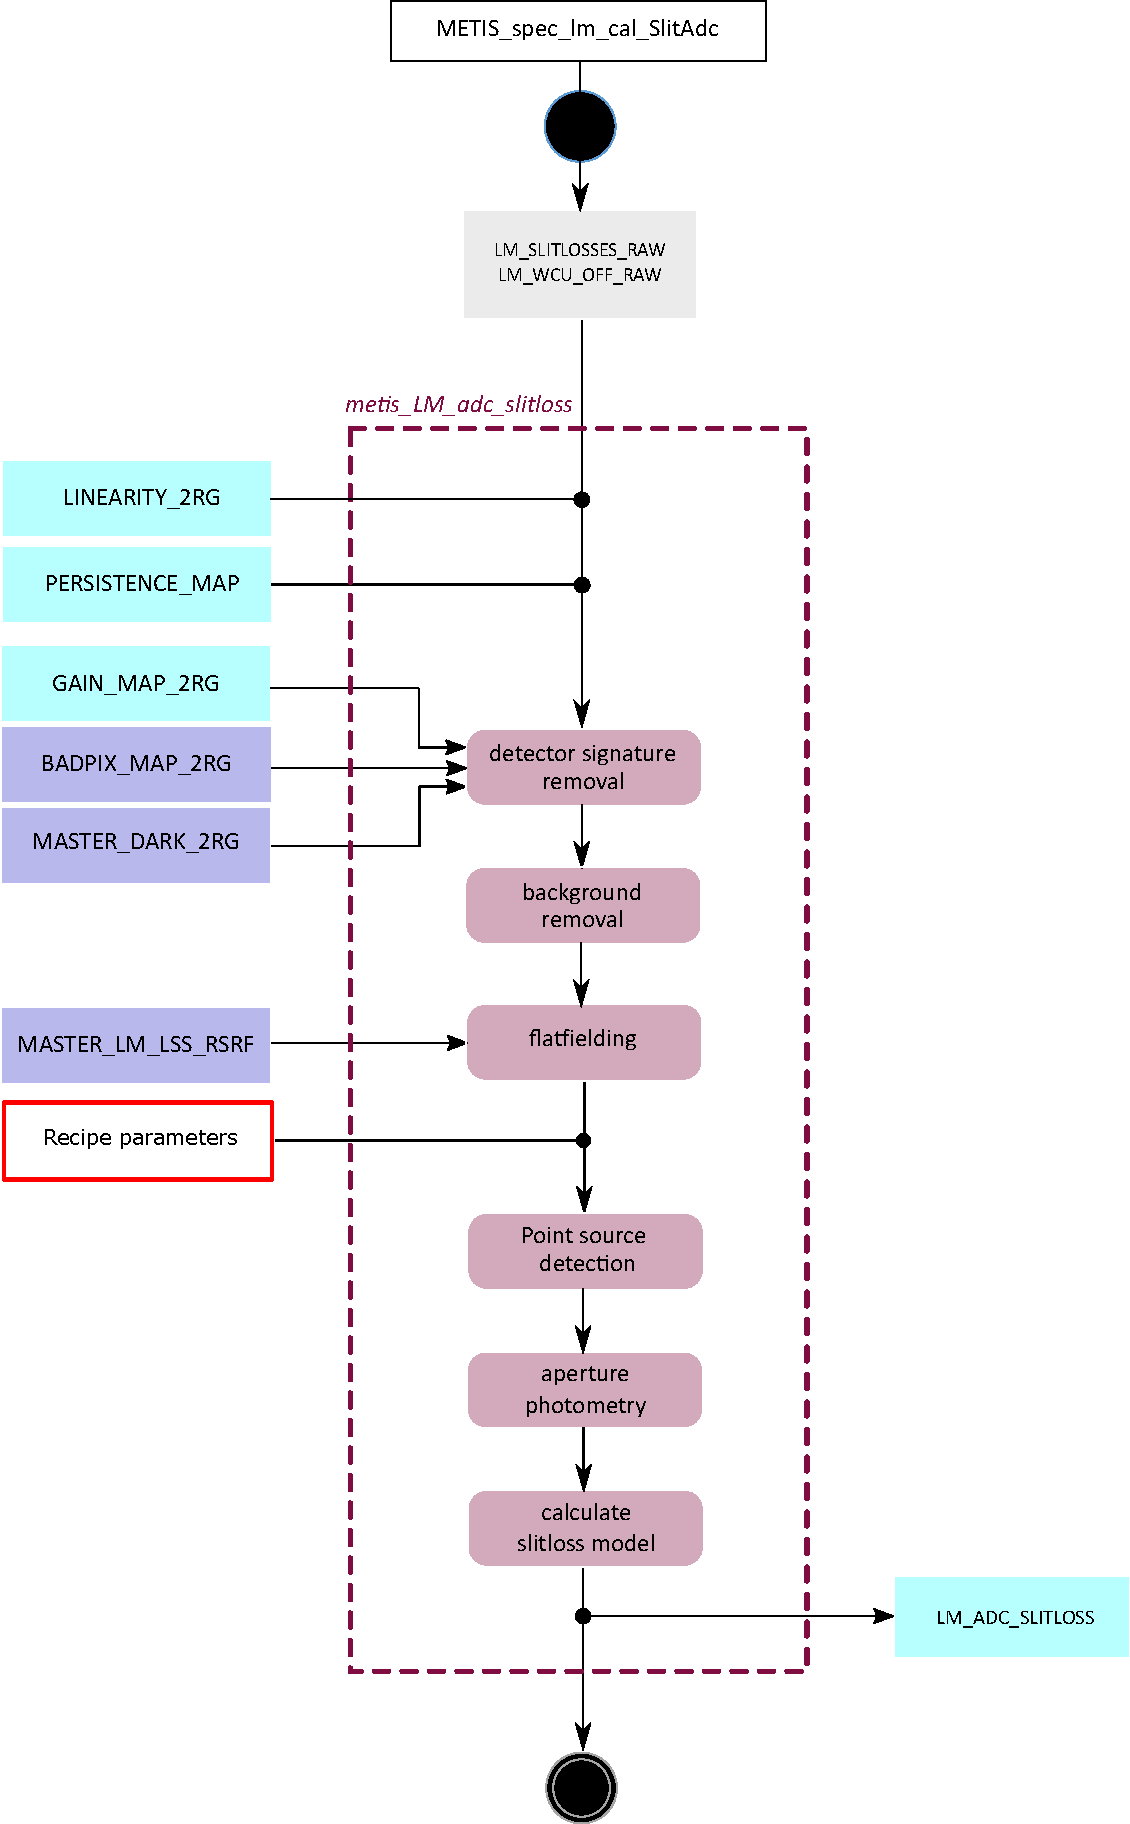
\includegraphics[width=0.5\textheight]{figures/metis_lm_adc_slitloss_v0.83.pdf}
    \notgenerated{flowchart: hand-drawn; the recipe declares no steps}
  \caption[Recipe: \REC*{metis_lm_adc_slitloss}]{\REC*{metis_lm_adc_slitloss} --
    Recipe workflow to determine the \ac{ADC} induced slit losses.}
  \label{Fig:rec_lm_adc_slitloss}
\end{figure}

\begin{recipedef}
  Name:                & \REC{metis_lm_adc_slitloss} \\
  Purpose:             & Determines ADC slitlosses \\
%  Requirements:        & \REQ{METIS-XXXX} \\
%  Type:                & Calibration | Science | Technical \\
%  Templates:           & \TPL{...} \\
  Primary input:       & \RAW{LM_ADC_SLITLOSS_RAW} (1--N) \\
                       & \RAW{LM_WCU_OFF_RAW} (1--N) \\
  Secondary inputs:    & \PROD{BADPIX_MAP_2RG} (optional) \\
                       & \hyperref[dataitem:gain_map_det]{\STATCALIB*{GAIN_MAP_2RG}} \\
                       & \hyperref[dataitem:linearity_det]{\PROD*{LINEARITY_2RG}} \\
                       & \PROD{MASTER_DARK_2RG} \\
                       & \EXTCALIB{PERSISTENCE_MAP} (optional) \\
  Matched keywords:    & \FITS{DET.DIT} \\
                       & \FITS{DET.NDIT} \\
                       & \FITS{DRS.SLIT} \\
  Parameters:          & \CODE{metis_lm_adc_slitloss.parameter1}\newline Description of parameter 1 (\texttt{value2}, \texttt{value1}), default \texttt{value1} \\
  Algorithm:           & Incredible fancy description of algorithm follows... ***TBD*** \\
  Output data:         & \STATCALIB{LM_ADC_SLITLOSS} \\
%  Expected accuracies: & \\
  QC1 parameters:      & --- none --- \\
\end{recipedef}


\label{rec:metislmadcmslitloss}
\label{rec:metis_lm_adc_slitloss}


\begin{figure}[ht]
  \centering
  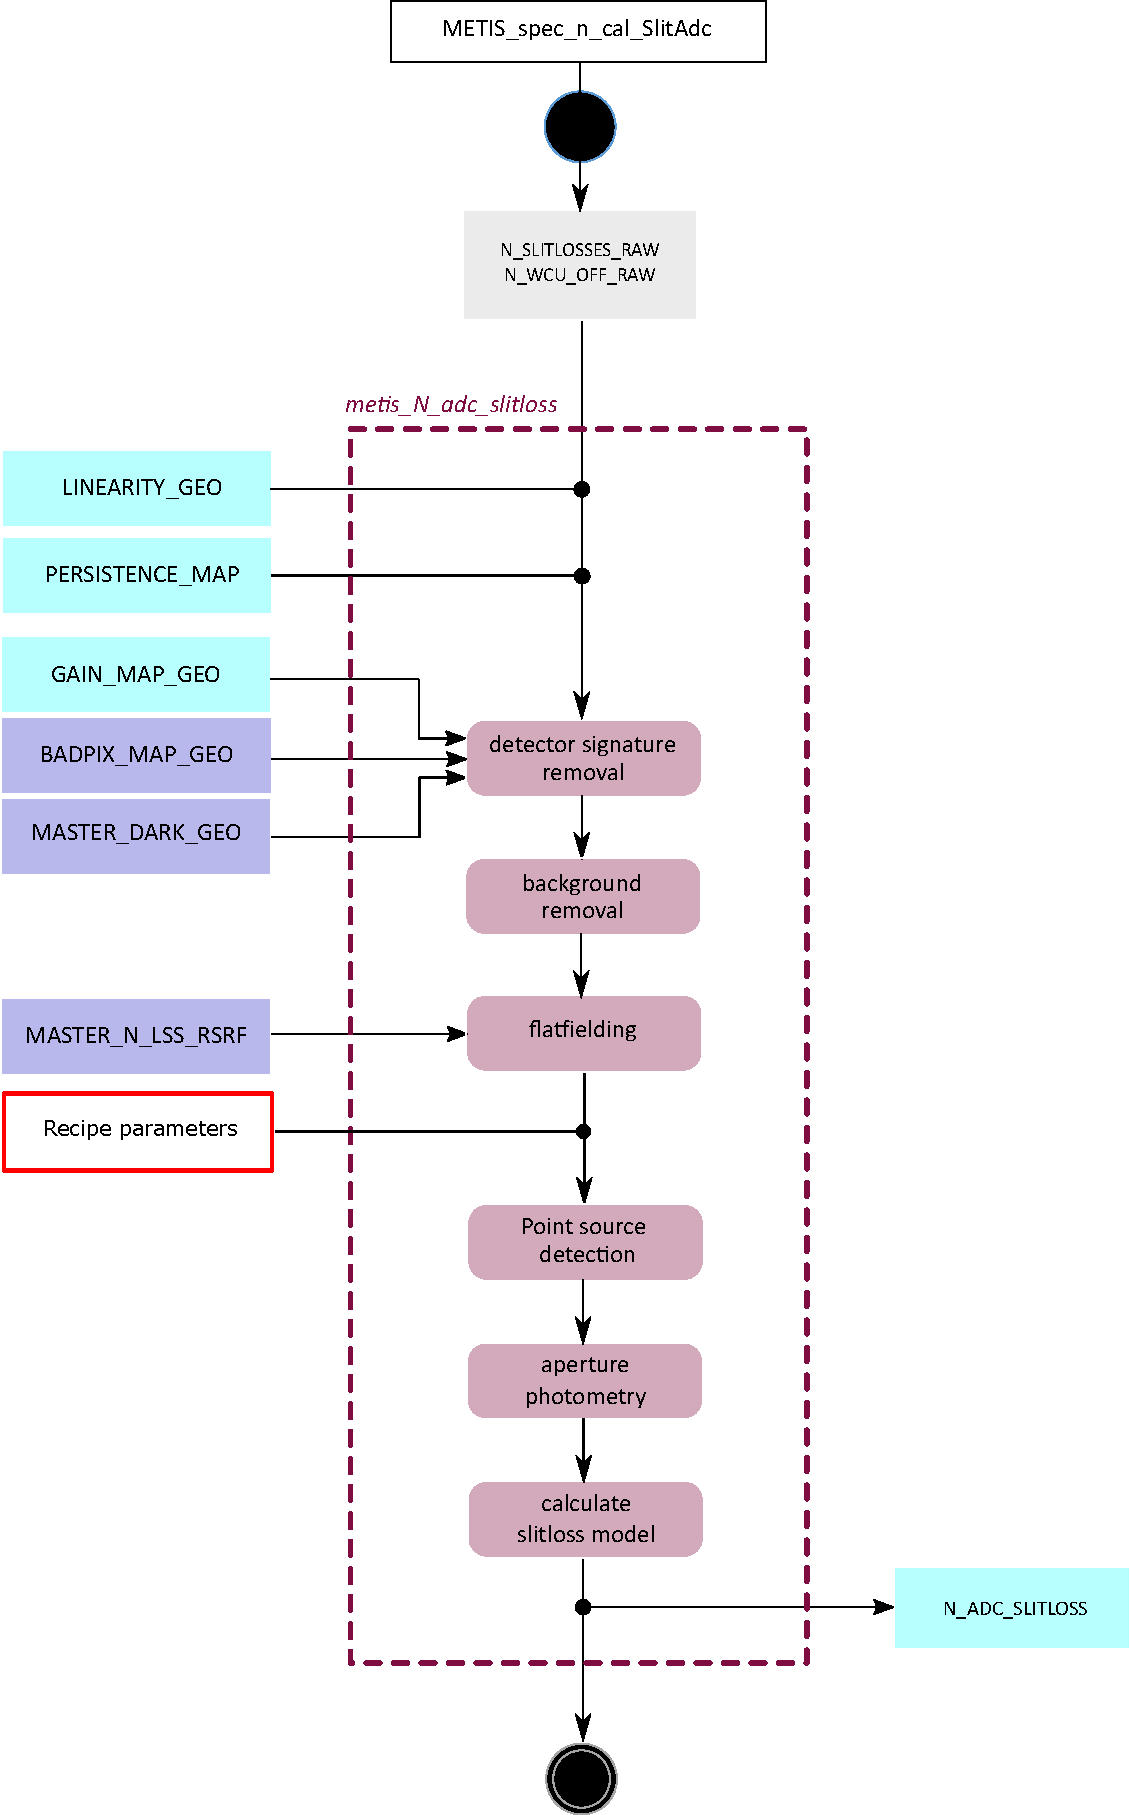
\includegraphics[width=0.5\textheight]{figures/metis_n_adc_slitloss_v0.83.pdf}
    \notgenerated{flowchart: hand-drawn; the recipe declares no steps}
  \caption[Recipe: \REC*{metis_n_adc_slitloss}]{\REC*{metis_n_adc_slitloss} --
    Recipe workflow to determine the \ac{ADC} induced slit losses.}
  \label{Fig:rec_n_adc_slitloss}
\end{figure}

\begin{recipedef}
  Name:                & \REC{metis_n_adc_slitloss} \\
  Purpose:             & Determines ADC slitlosses \\
%  Requirements:        & \REQ{METIS-XXXX} \\
%  Type:                & Calibration | Science | Technical \\
%  Templates:           & \TPL{...} \\
  Primary input:       & \RAW{N_ADC_SLITLOSS_RAW} (N$\times$) \\
                       & \RAW{N_WCU_OFF_RAW} (N$\times$) \\
  Secondary inputs:    & \PROD{BADPIX_MAP_GEO} (optional) \\
                       & \hyperref[dataitem:gain_map_det]{\STATCALIB*{GAIN_MAP_GEO}} \\
                       & \hyperref[dataitem:linearity_det]{\PROD*{LINEARITY_GEO}} \\
                       & \PROD{MASTER_DARK_GEO} \\
                       & \EXTCALIB{PERSISTENCE_MAP} (optional) \\
  Matched keywords:    & \FITS{DET.DIT} \\
                       & \FITS{DET.NDIT} \\
                       & \FITS{DRS.SLIT} \\
  Parameters:          & \CODE{metis_n_adc_slitloss.parameter1}\newline Description of parameter 1 (\texttt{value2}, \texttt{value1}), default \texttt{value1} \\
  Algorithm:           & Incredible fancy description of algorithm follows... ***TBD*** \\
  Output data:         & \STATCALIB{N_ADC_SLITLOSS} \\
%  Expected accuracies: & \\
  QC1 parameters:      & --- none --- \\
\end{recipedef}


\label{rec:metisnadcmslitloss}
\label{rec:metis_n_adc_slitloss}

%------------------------------------------------------------------------------------------------------------------
\subsubsection{Fringing correction}
\label{rec:metis_fringing_correction}

It is unclear for the time being how much of a problem will be with the METIS
detectors, and what the best strategy will be to tackle it. Therefore, the
method to use will be chosen based on AIT results (\REQ{METIS-9151}, for rationale and basic method description see Ch.~3.12 in the Calibration Plan~\cite{METIS-calibration_plan}).

Whether a stand-alone recipe will be required, or if the fringe-map will become
part of another recipe, is part of that uncertainty. If needed, the design of
said recipe will be minimal work and is thus omitted in this document.

%%% Local Variables:
%%% mode: latex
%%% TeX-master: "METIS_DRLD"
%%% End:
